\chapter{XBee}
\label{cha:XBee}

\section{ZigBee模块概述}

无线电通信协议是在无线电设备之间进行数据交换的一组规则。RF模块根据模块及其无线电固件支持特定的无线电通信协议。

以下是XBee无线电模块支持的协议的完整列表:

\begin{itemize}
    \item IEEE 802.15.4
    \item ZigBee
    \item ZigBee Smart Energy
    \item DigiMesh (Digi proprietary)
    \item ZNet
    \item IEEE 802.11 (Wi-Fi)
    \item Point-to-multipoint (Digi proprietary)
    \item XSC (XStream-compatible)
\end{itemize}

\begin{figure}[htbp]
    \centering
    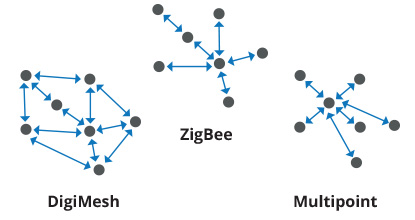
\includegraphics[width=0.5\columnwidth]{radio_comm_protocols.png}
    \caption{不同协议组网方式对比}
    \label{fig:radio_comm_protocols}
\end{figure}

并非所有XBee设备都可以运行所有列出的通信协议。XBee硬件和无线电固件的组合决定了XBee设备可以执行的协议。

\section{固件升级}

本地设备设置AP=2 即 API mode 能使用Network Working Mode,以便升级固件。

用XBee 3 无线连接淘宝买的XBee Pro S2B需要先下载lagacy XBee Firmware。但不能直接无线更新固件,还是需要用USB连接到电脑上烧写新固件。XBee3则可以直接无线更新。

这就决定了小车上尽可能使用XBee3,虽然要比XBee S2B贵3-4倍。当然也可以直接在我们的PCB上画FT232接USB口以便更新固件使用,或者预留编程口直接使用编程线。

只有以下这些模块才能无线更新固件:

\begin{itemize}
    \item XBee/XBee PRO SX
    \item XLR Pro Module
    \item XBee/XBee PRO 802.15.4 (S2C module versions only)
    \item XBee/XBee-PRO DigiMesh 2.4 (S2C module versions only)
    \item XTend RF Module Family (SX module versions only)
    \item XBee/XBee-PRO ZB and Programmable XBee-PRO ZB
    \item XBee/XBee-PRO ZB SMT and Programmable XBee-PRO ZB SMT
    \item XBee-PRO 900HP and Programmable XBee-PRO 900HP
    \item XBee 865LP and Programmable XBee 865LP
    \item XBee3 (Zigbee, DigiMesh 2.4, and 802.15.4)
\end{itemize}

\section{AP参数}

XBee无线电模块的操作模式建立了用户或连接到XBee的任何微控制器通过通用异步接收器/发送器(UART)或串行接口与模块进行通信的方式。

取决于固件及其配置,无线电模块可以在三种不同的操作模式下工作:

\begin{itemize}
    \item Application Transparent (AT) operating mode
    \item API operating mode
    \item API escaped operating mode
\end{itemize}

在某些情况下,无线电模块的运行模式由固件版本(确定运行模式是AT还是API)以及固件的AP设置(确定API模式是否被转义(2))建立, (1)。在其他情况下,操作模式仅由AP设置确定,该设置允许您将模式配置为AT(AP = 0),API(AP = 1)或API转义(AP = 2)。
\section{AT设置}

